
\subsection{Построение карты поверхности}


\subsubsection{Теория}


\begin{figure}[H]
    \centering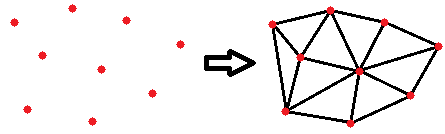
\includegraphics[height=6cm,width=1\textwidth,keepaspectratio]{delone_idea.png}
    \caption*{Common 2D Delaunay triangulation (Convex Hull) \\ \textbf{From Point Cloud to mesh}}
    \label{fig:delone_idea.png}
\end{figure}

\begin{figure}[H]
    \begin{subfigure}[t]{0.49\textwidth}
        \centering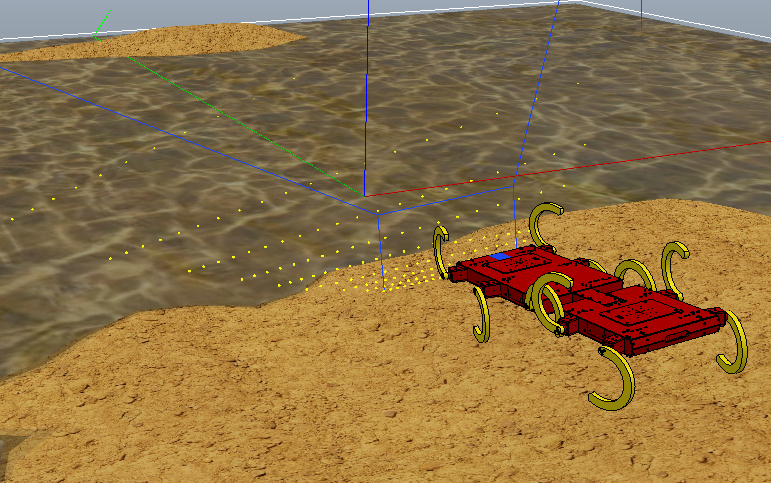
\includegraphics[height=5cm,width=1\textwidth,keepaspectratio]{terrain_w_water1.png}
        \caption*{Start point}
    \end{subfigure}
    \begin{subfigure}[t]{0.49\textwidth}
        \centering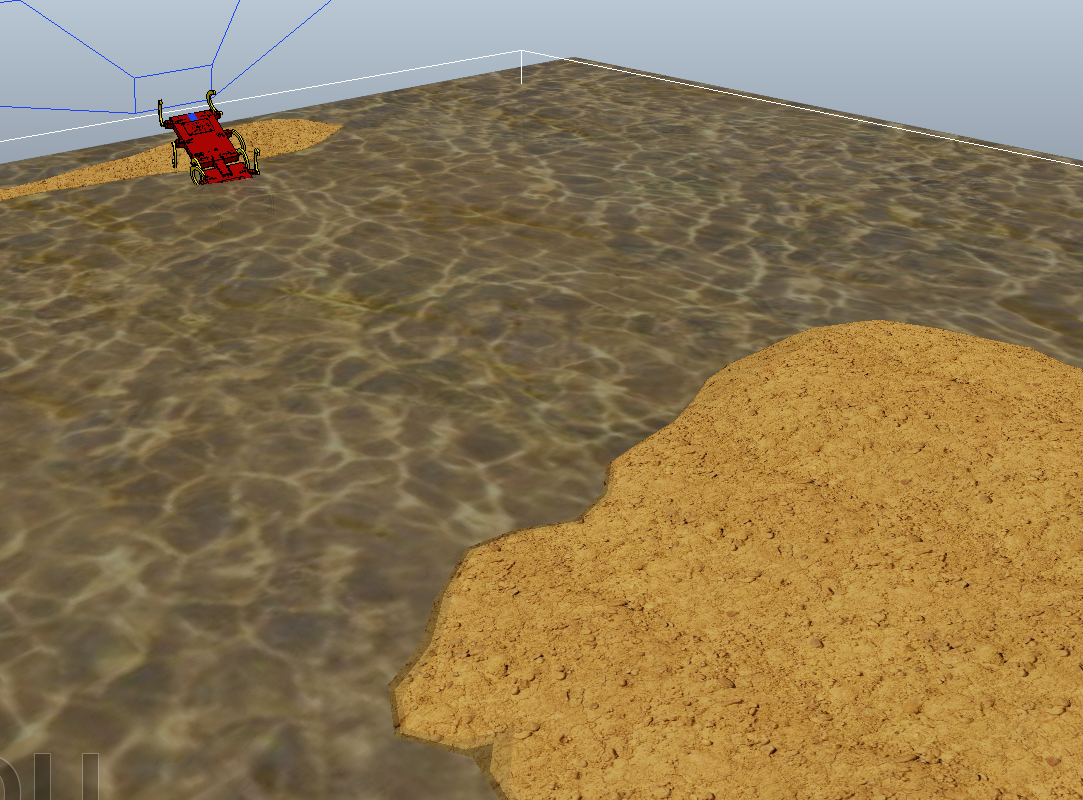
\includegraphics[height=5cm,width=1\textwidth,keepaspectratio]{terrain_w_water_end.png}
        \caption*{End point}
    \end{subfigure}
\end{figure}

\begin{figure}[H]
    \begin{subfigure}[t]{0.49\textwidth}
        \centering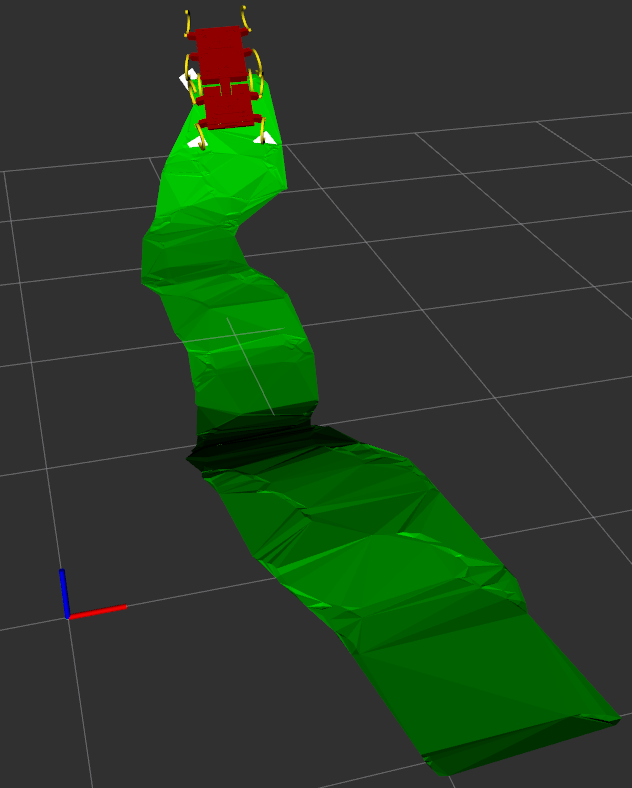
\includegraphics[height=5cm,width=1\textwidth,keepaspectratio]{mesh_rviz.png}
        \caption*{Mesh created using concave hull 2D Delaunay triangulation}
    \end{subfigure}
    \begin{subfigure}[t]{0.49\textwidth}
            \centering
             \begin{tikzpicture}
                % Include the image in a node
                \node [above right, inner sep=0] (image) at (0,0) 
                {\centering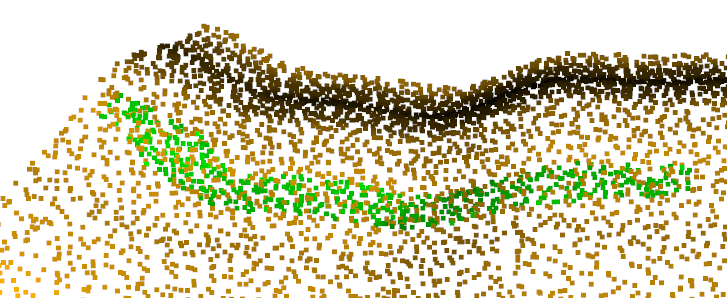
\includegraphics[height=5cm,width=1\textwidth,keepaspectratio]{sampled_pcd.png}};          
                % Create scope with normalized axes
                \begin{scope}[
                    x={($ 0.1*(image.south east)$)},
                    y={($ 0.1*(image.north west)$)}]
                    % Grid and axes' labels
                    % \draw[lightgray,step=1] (image.south west) grid (image.north east);
                    % \foreach \x in {0,1,...,10} { \node [below] at (\x,0) {\x}; }
                    % \foreach \y in {0,1,...,10} { \node [left] at (0,\y) {\y};}
         
                    % Labels
                    \draw[stealth-, very thick,green] (3,8) -- (2,8.5);
                    \draw[stealth-, very thick,green] (1,5.5) -- (2,8.5)
                    node[rounded corners=3pt,above,black,fill=white]{\tiny Ground Truth Point Cloud};
         
                    \draw[stealth-, very thick,green] (5.5,3) -- (5.5,8.5)
                    node[rounded corners=3pt,above,black,fill=white]{\tiny Generated Point Cloud};
                \end{scope}
            \end{tikzpicture}
            \caption*{Sampled point cloud}
            \label{fig:sampled_pcd.png}
    \end{subfigure}
\end{figure}

\begin{figure}[H]
    \begin{subfigure}[t]{0.3\textwidth}
        \centering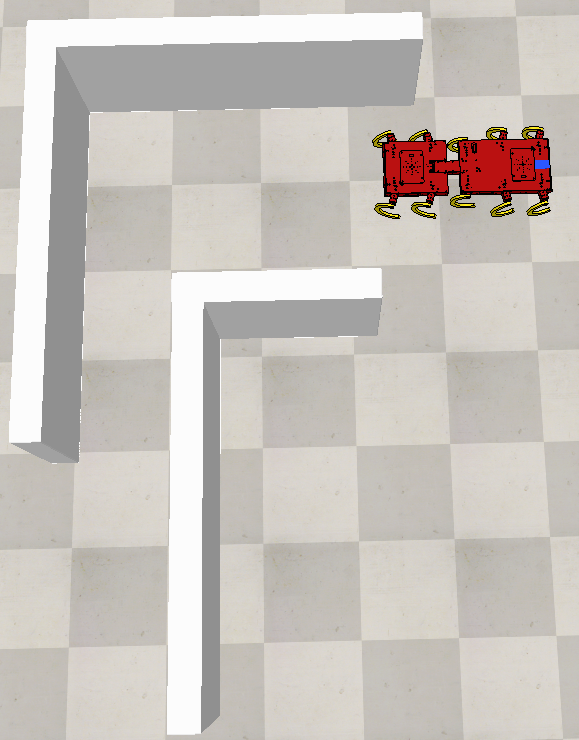
\includegraphics[height=5cm,width=1\textwidth,keepaspectratio]{convex_terr.png}
        \caption*{Case study}
        \label{fig:convex_terr.png}
    \end{subfigure}
    \hfill
    \begin{subfigure}[t]{0.33\textwidth}
            \centering
             \begin{tikzpicture}
                % Include the image in a node
                \node [above right, inner sep=0] (image) at (0,0) 
                {\centering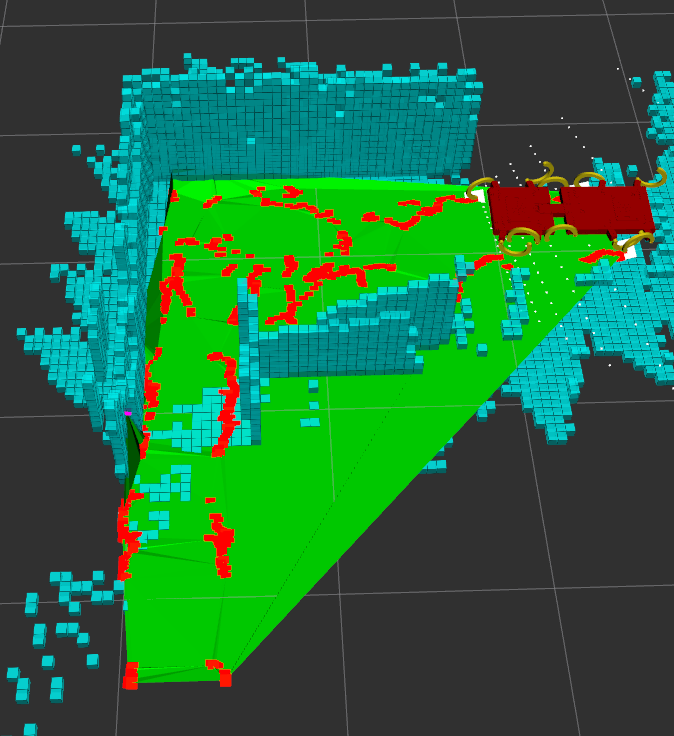
\includegraphics[height=6cm,width=1\textwidth,keepaspectratio]{conv_convex.png}};          
                % Create scope with normalized axes
                \begin{scope}[
                    x={($ 0.1*(image.south east)$)},
                    y={($ 0.1*(image.north west)$)}]
                    % Grid and axes' labels
                    % \draw[lightgray,step=1] (image.south west) grid (image.north east);
                    % \foreach \x in {0,1,...,10} { \node [below] at (\x,0) {\x}; }
                    % \foreach \y in {0,1,...,10} { \node [left] at (0,\y) {\y};}
         
                    % Labels
                    \draw[stealth-, very thick,green] (5.2,3.5) -- ++(1,-1)
                    node[rounded corners=3pt,right,black,fill=white]{\tiny Generated mesh};
                    
                    \draw[stealth-, very thick,green] (5.5,5.5) -- (7.4,4)
                    node[rounded corners=3pt,right,black,fill=white]{\tiny Lidar data};
                    
                    
                    \draw[stealth-, very thick,green] (3.4,0.8) -- (5,1);            
                    \draw[stealth-, very thick,green] (3.4,2.6) -- (5,1)
                    node[rounded corners=3pt,right,black,fill=white]{\tiny Cloud of contact points};
                \end{scope}
            \end{tikzpicture}
            \caption*{Convex Hull}
            \label{fig:conv_convex.png}
    \end{subfigure}
    \hfill
    \begin{subfigure}[t]{0.33\textwidth}
        \centering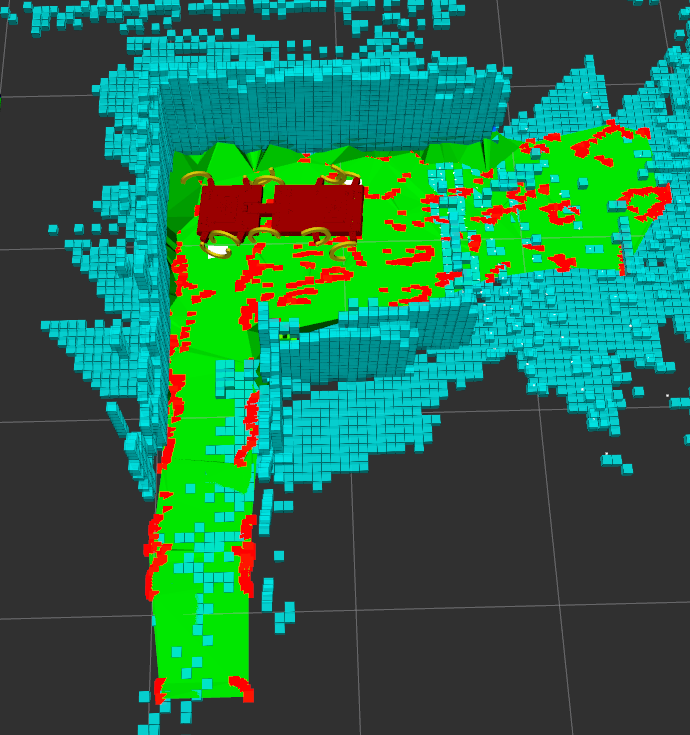
\includegraphics[height=6cm,width=1\textwidth,keepaspectratio]{conv_concave.png}
        \caption*{Concave Hull}
        \label{fig:conv_concave.png}
    \end{subfigure}

\end{figure}

\begin{figure}[H]
    \begin{subfigure}[t]{0.49\textwidth}
        \centering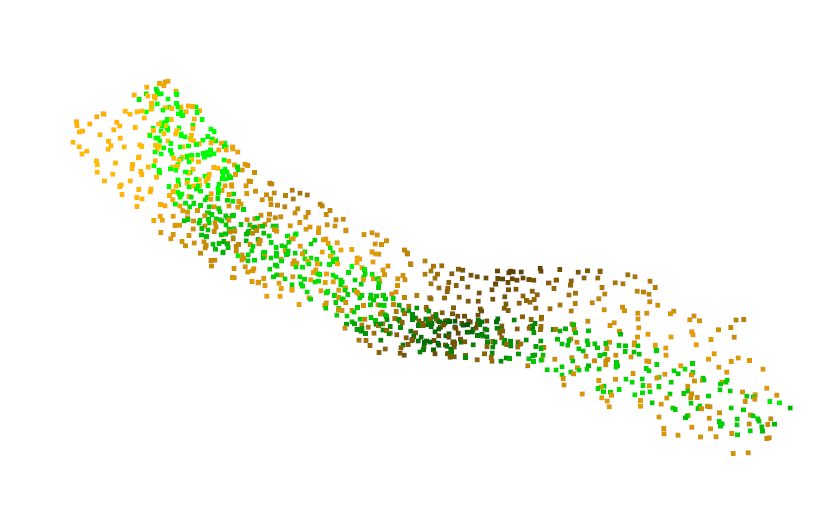
\includegraphics[height=5cm,width=1\textwidth,keepaspectratio]{cropped_pcd.png}
        \caption*{Overlaid Point Clouds}
    \end{subfigure}
    \begin{subfigure}[t]{0.49\textwidth}
        \centering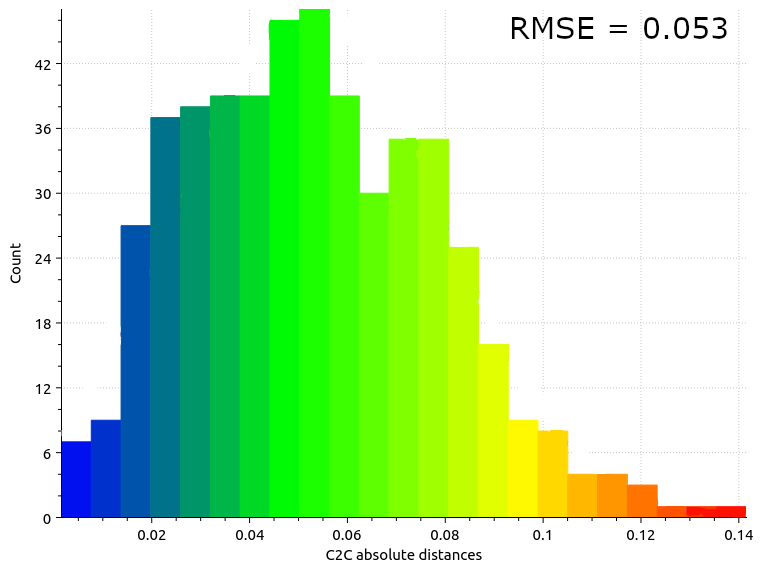
\includegraphics[height=5cm,width=1\textwidth,keepaspectratio]{pcd_hist.png}
        \caption*{Error histogram (distance from a point to closest ground truth point)}
    \end{subfigure}
\end{figure}

\begin{figure}[H]
    \begin{subfigure}[t]{0.49\textwidth}
        \centering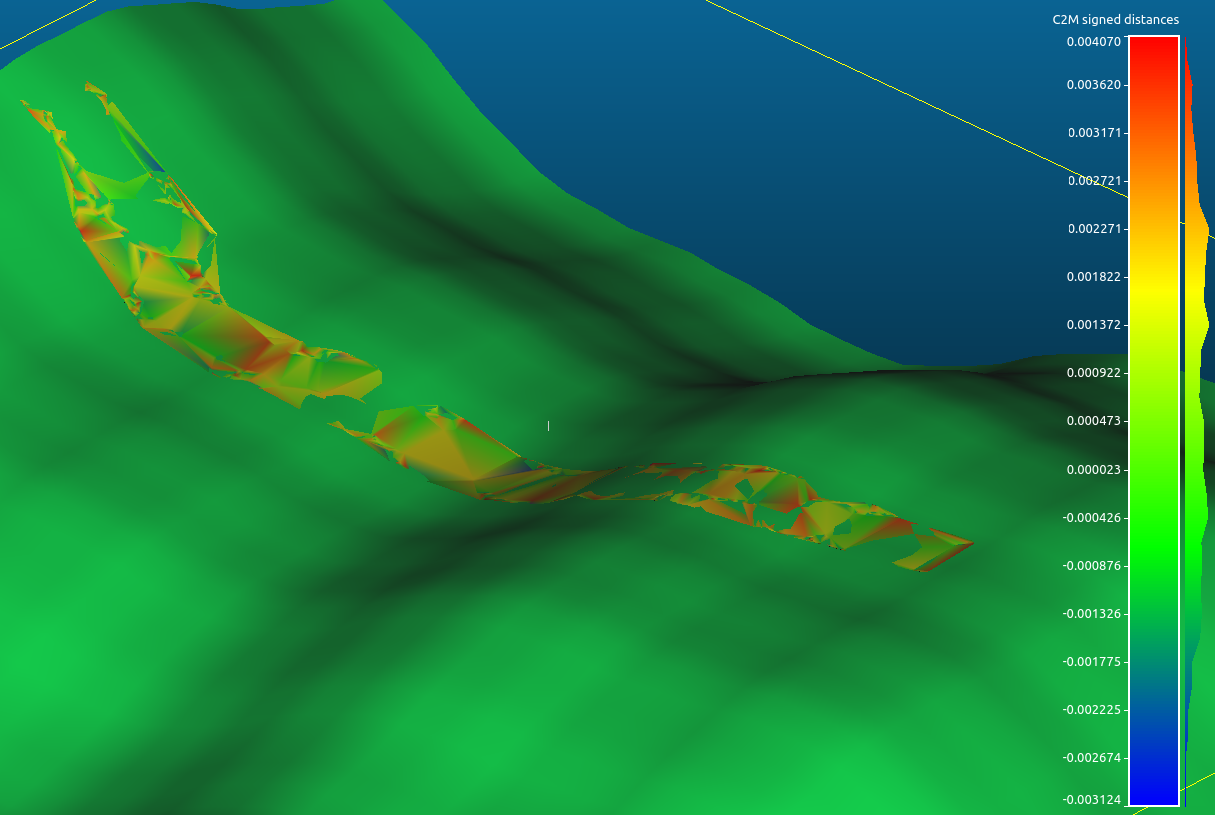
\includegraphics[height=5cm,width=1\textwidth,keepaspectratio]{mesh_comp.png}
        \caption*{Overlaid Meshes}
    \end{subfigure}
    \begin{subfigure}[t]{0.49\textwidth}
        \centering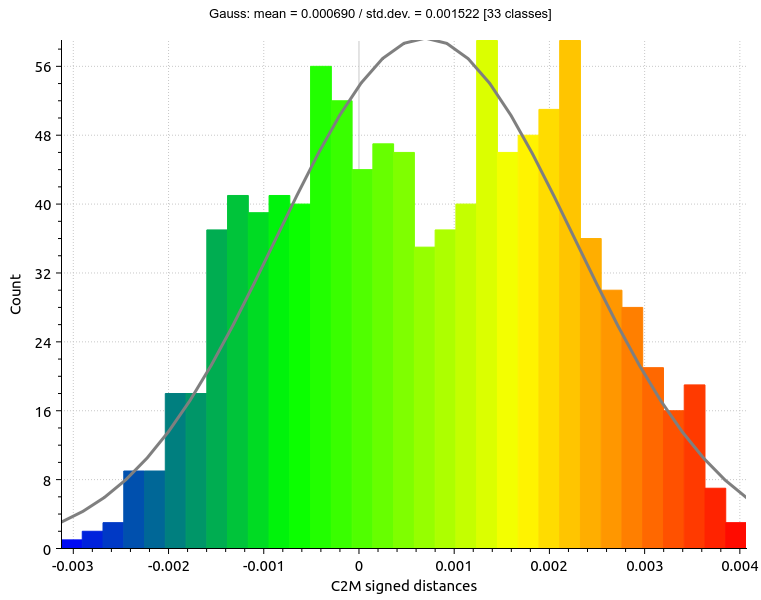
\includegraphics[height=5cm,width=1\textwidth,keepaspectratio]{mesh_hist.png}
        \caption*{Error histogram (distance from a point to closest ground truth point)}
    \end{subfigure}
\end{figure}

\begin{figure}[H]
    \begin{subfigure}[t]{0.49\textwidth}
        % \href{run:./videos/big_angle2.mp4}{
        \href{https://youtu.be/2dxHHTG4psQ}{
            \centering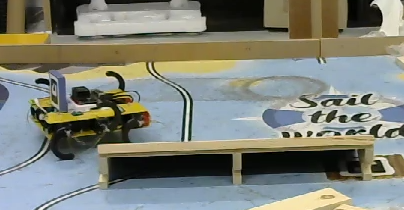
\includegraphics[height=6cm,width=1\textwidth,keepaspectratio]{real_robot_mesh_video_preview.png}}
        \caption*{Robot is passing the obstacle}
    \end{subfigure}
    \begin{subfigure}[t]{0.49\textwidth}
        \centering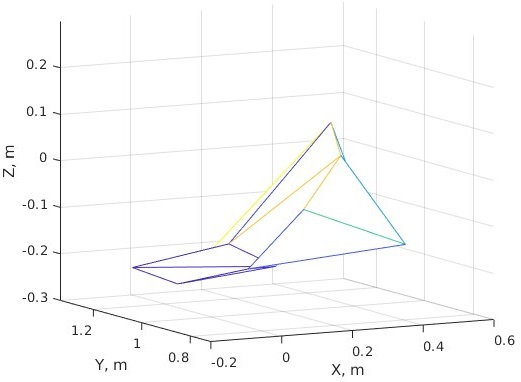
\includegraphics[height=6cm,width=1\textwidth,keepaspectratio]{real_mesh.jpg}
        \caption*{Mesh, obtained from legs}
    \end{subfigure}
\end{figure}

текст

Расписываю текущую работу. Уверен, что там будет доп подглавы.


\subsection{Определение типа поверхности}

Для нужно

\begin{figure}[H]
    \begin{subfigure}[t]{0.49\textwidth}
        \centering
        \begin{tikzpicture}
            % Include the image in a node
            \node [above right, inner sep=0] (image) at (0,0)
            {\centering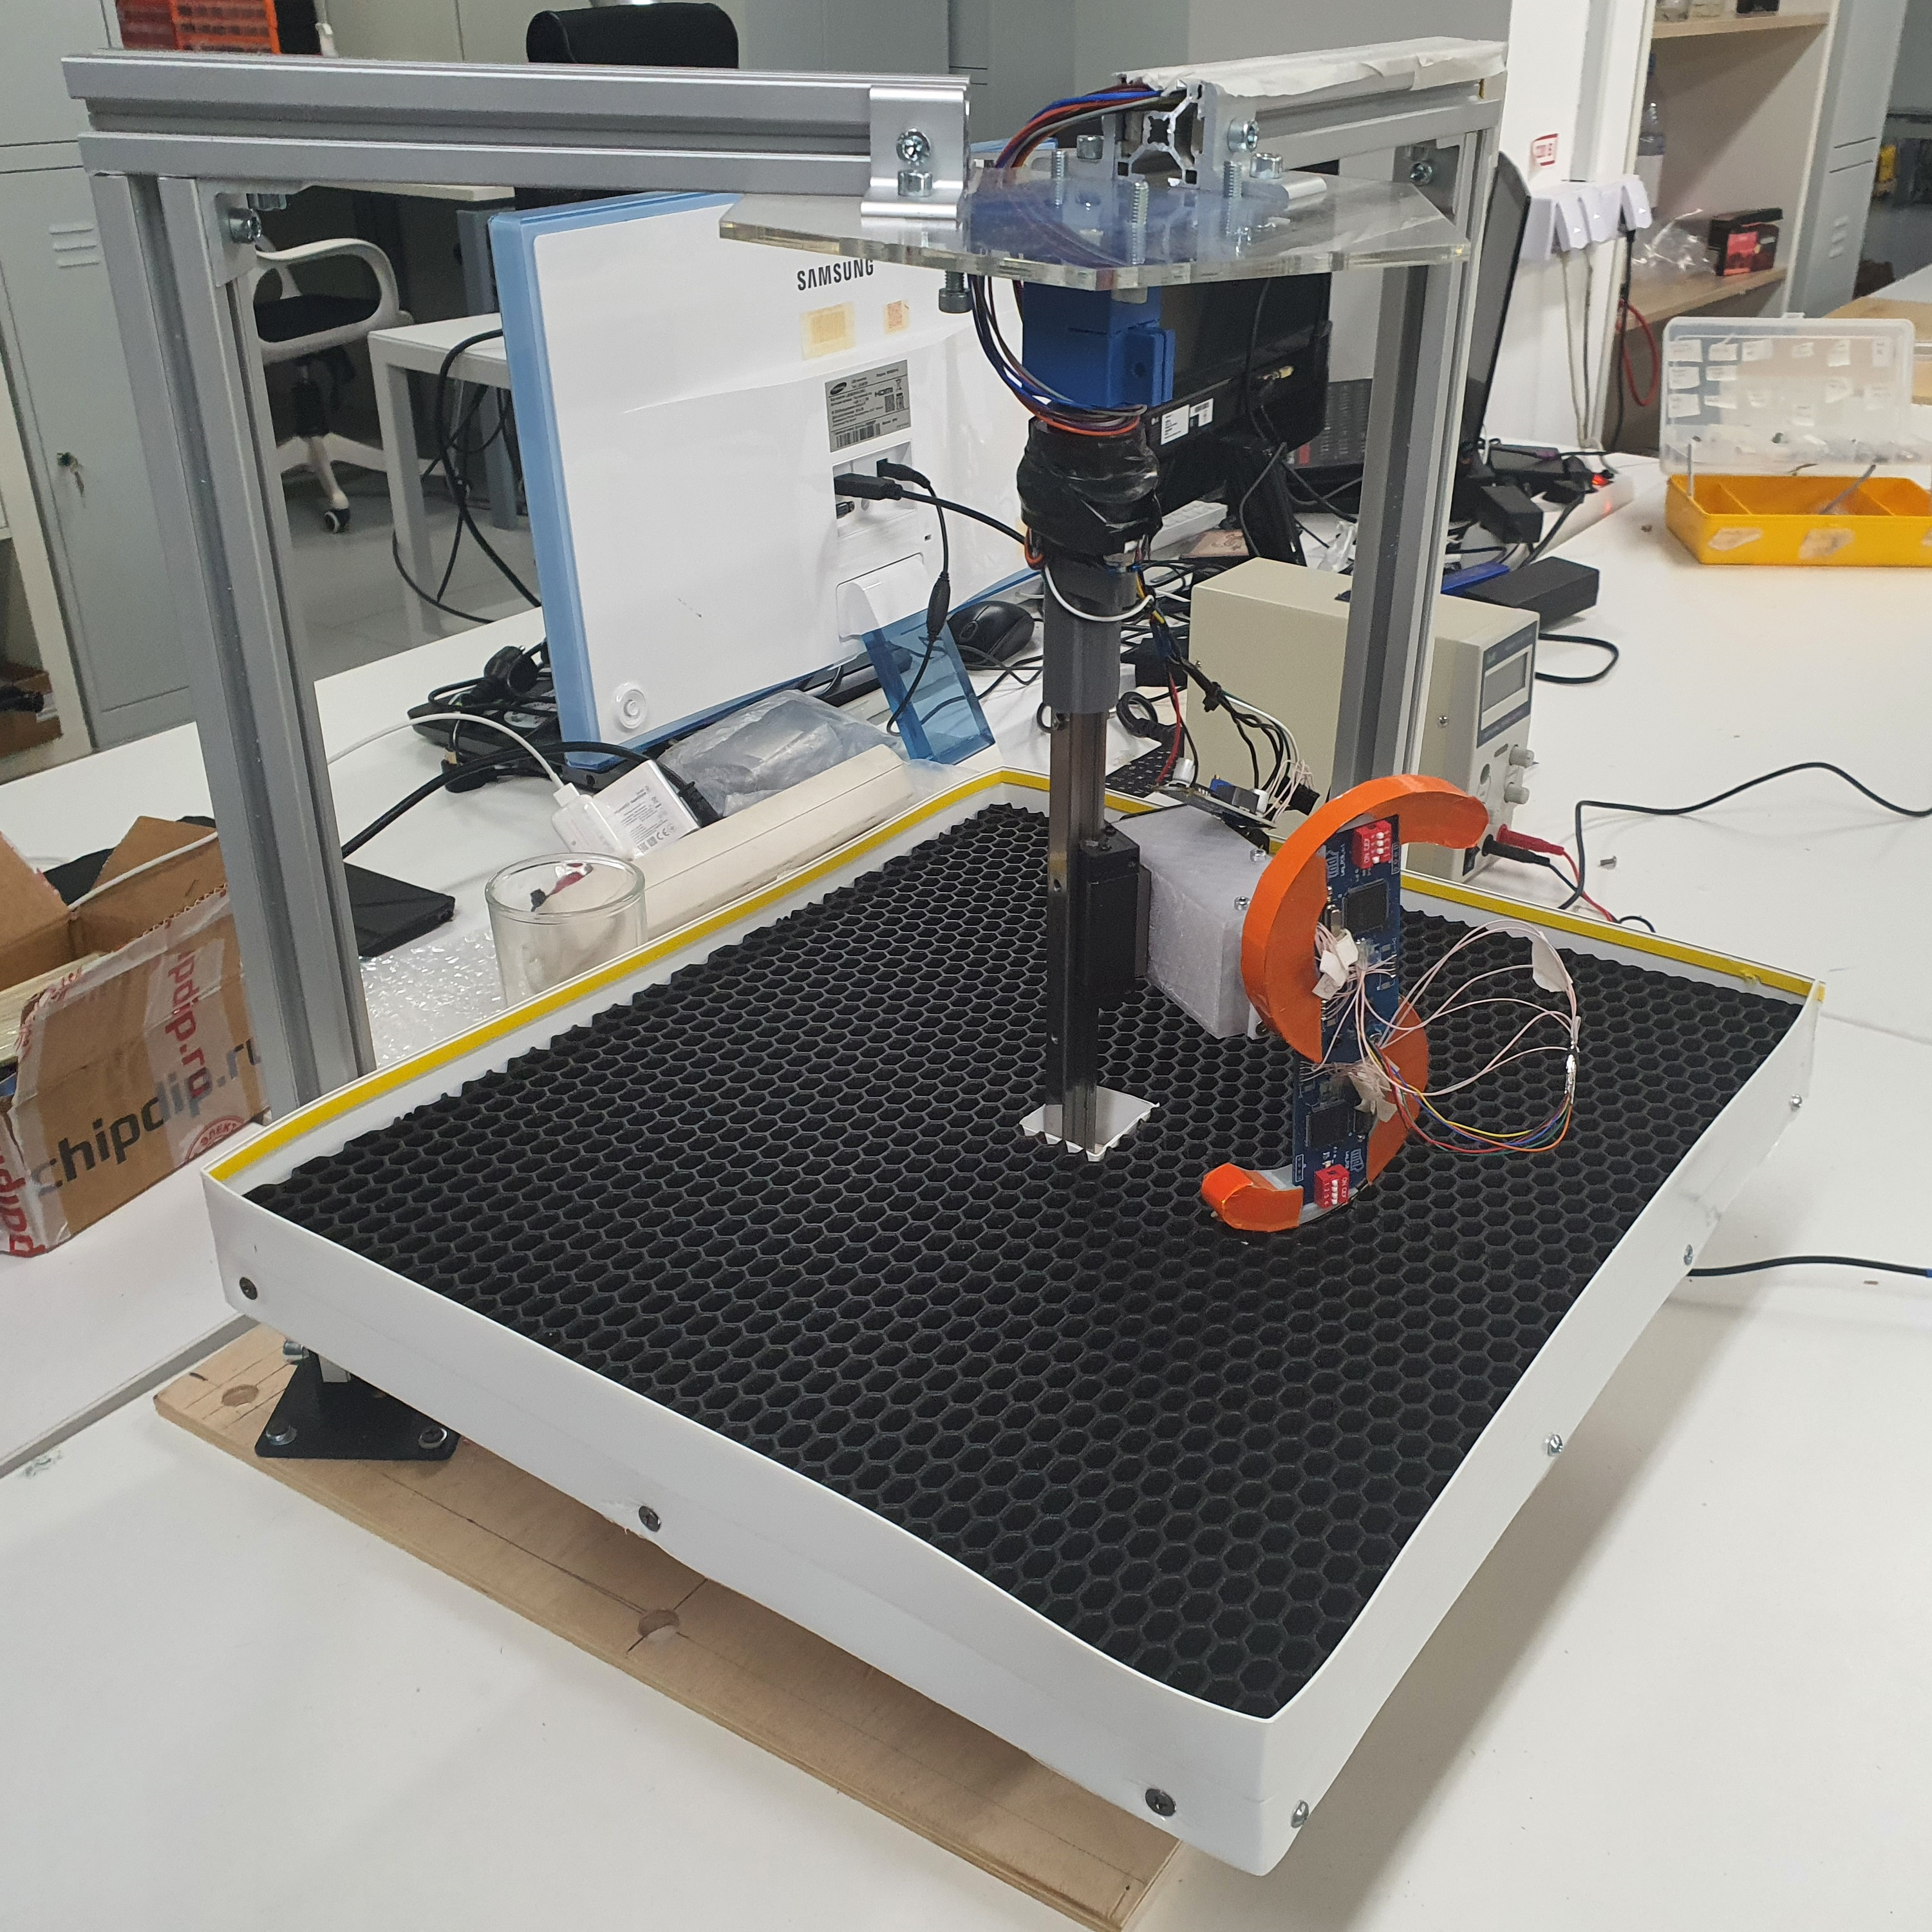
\includegraphics[height=6cm,width=1\textwidth,keepaspectratio]{s_shape_leg/s_leg_setup.JPG}};
            % Create scope with normalized axes
            \begin{scope}[
                    x={($ 0.1*(image.south east)$)},
                    y={($ 0.1*(image.north west)$)}]
                \draw[stealth-, very thick,green] (3.5,2.5) -- (3,1.5)
                node[rounded corners=3pt,below,black,fill=white]{\tiny Table for surfaces};

                \draw[stealth-, very thick,green] (7.1,5.4) -- (7.4,7)
                node[rounded corners=3pt,above right,black,fill=white]{\tiny Self-made PCB};

                \draw[very thick,green] (6,6.1) rectangle (8.5,3.5)
                node[above left,black,fill=green]{\tiny S leg};
            \end{scope}
        \end{tikzpicture}
        \caption{Общий вид экспериментальной установки}
        \label{fig:s_shape_leg/s_leg_setup.JPG}
    \end{subfigure}
    \begin{subfigure}[t]{0.49\textwidth}
        \centering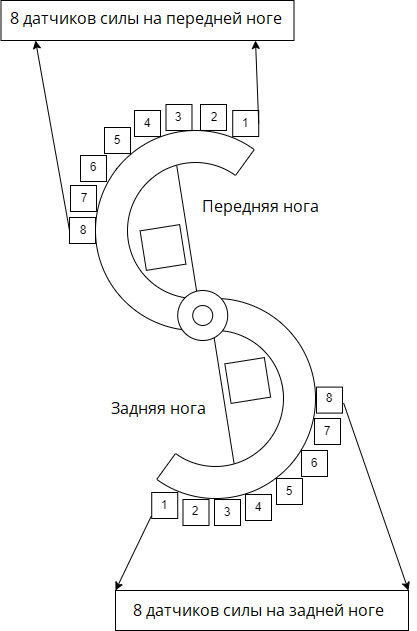
\includegraphics[height=6cm,width=1\textwidth,keepaspectratio]{s_shape_leg/leg_design.png}
        \caption{Пояснение по расположению сенсоров на ноге робота}
        \label{fig:s_shape_leg/leg_design.png}
    \end{subfigure}
    \caption{Экспериментальная установка для определения типа поверхности}
\end{figure}

Текст текст

\begin{figure}[H]
    \begin{subfigure}{0.49\textwidth}
        \centering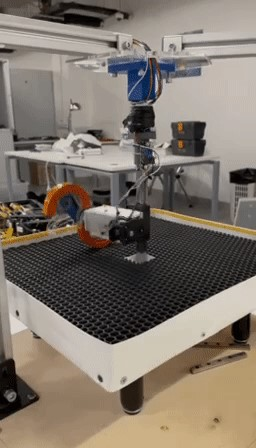
\includegraphics[height=6cm,width=1\textwidth,keepaspectratio]{s_shape_leg/flat.jpg}
        \caption{Резина}
        \label{fig:s_shape_leg/flat.jpg}
    \end{subfigure}
    \hfill
    \begin{subfigure}{0.49\textwidth}
        \centering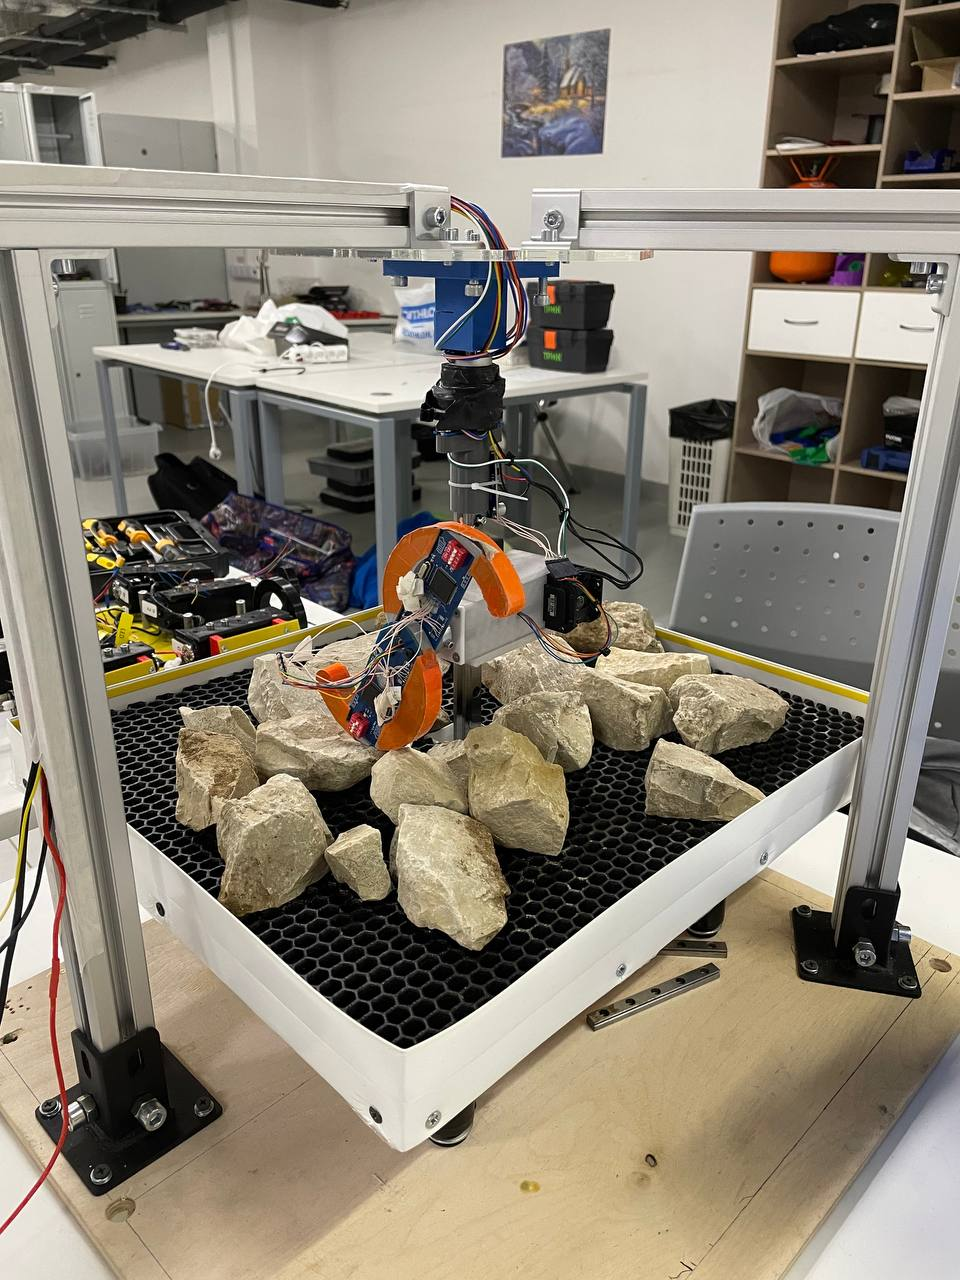
\includegraphics[height=6cm,width=1\textwidth,keepaspectratio]{s_shape_leg/view.jpg}
        \caption{Каменистая поверхность}
        \label{fig:s_shape_leg/view.jpg}
    \end{subfigure}
    \caption{Типы определяемых поверхностей}
\end{figure}

Из-за большого гистерезиса и трудностью с калибровкой необходимо работать с относительными данными.

\begin{figure}[H]
    \begin{subfigure}{0.49\textwidth}
        \centering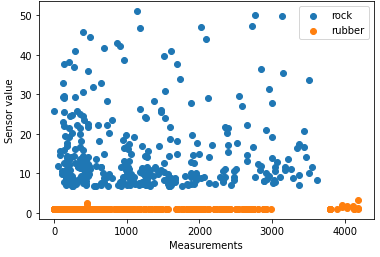
\includegraphics[height=3.8cm,width=1\textwidth,keepaspectratio]{s_shape_leg/segment8_compare_front.png}
        \caption{Передняя часть ноги, 8ой сегмент}
    \end{subfigure}
    \begin{subfigure}{0.49\textwidth}
        \centering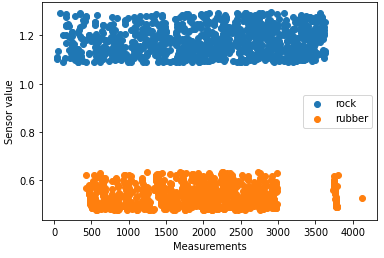
\includegraphics[height=3.8cm,width=1\textwidth,keepaspectratio]{s_shape_leg/segment6_compare_front.png}
        \caption{Передняя часть ноги, 6ой сегмент}
    \end{subfigure}
    \caption{Сравнение сырых данных после эксперимента с разных сегментов ноги}
    \label{fig:data_from_legs}
\end{figure}

На данный момент возможно явно различать резину и каменистую поверхность. Более того было доказано, что разработанный и исследованный преобразователь силы позволяет определять тип поверхности.